\documentclass{beamer}
\usepackage{tikz}
\usepackage{lmodern}
\usepackage{mathtools}
\usepackage[backend=biber, style=authoryear]{biblatex}
\addbibresource{references.bib}



\newcommand\N{\mathbb{N}}

\title[Graph limits]{Graph limits and exchangeable random graphs}
\author{Miheer Dewaskar}
\institute[UNC]{ 
  Department of Statistics and Operations Research\\
  University of North Carolina, Chapel Hill
}

\date{STOR 831 : Nov 30th 2017}
\subject{STOR 831}

\newtheorem{thm}{Theorem}[section]

\begin{document}
  \frame{\titlepage}

  \begin{frame}
  \frametitle{Table of Contents}
  \tableofcontents
  \end{frame}

  \section{Graphs}
  \begin{frame}
    \frametitle{Graphs}
    \begin{columns}
      \column{.5\textwidth}
      	\begin{tikzpicture}
	  [scale=.5,auto=left,every node/.style={circle}]
	\node (n6) at (1,10) {6};
	\node (n4) at (4,8)  {4};
	\node (n5) at (8,9)  {5};
	\node (n1) at (11,8) {1};
	\node (n2) at (9,6)  {2};
	\node (n3) at (5,5)  {3};

	\foreach \from/\to in {n6/n4,n4/n5,n5/n1,n1/n2,n2/n5,n2/n3,n3/n4}
	  \draw (\from) -- (\to);
	\end{tikzpicture}	
      \column{.5\textwidth}
	\begin{description}
	  \item[Definition] $G=(V, E)$ for $E \subseteq V \times V$
	  \item[Simple] Undirected, no self loop or multiple edges.
	  \item[Notation] $|G| = |V|$ (at most countable).
	\end{description}
    \end{columns}

    \pause
    \bigskip
    \begin{block}{Applications}
      \begin{description}
	\item[Math] Fundamental objects in discrete math.
	\item[Statistical Physics] Crystals, magnetization. 
	\item[Large networks] Internet, social and biological networks. 
      \end{description}
    \end{block}
  \end{frame}
  \note{Applications deal with large networks with billions of nodes. Statistics on networks.
  The theory of graph limits address some of these issues.}

  \section{Graph limits}

  \begin{frame}
    \frametitle{Convergence Example}
    \begin{columns}
      \column{.6\textwidth}
	\begin{figure}
	  \centering
	  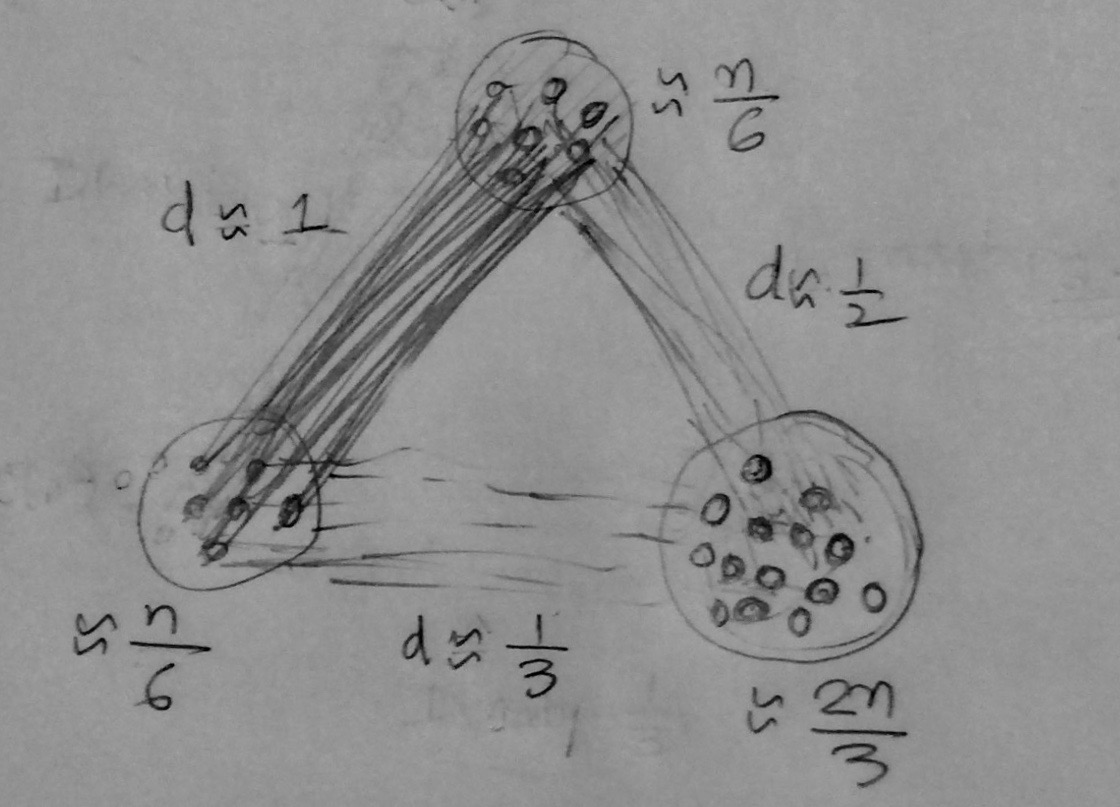
\includegraphics[totalheight=5cm]{./Images/Graphs.jpg}
	  \caption{$G_n$ on $n$ vertices (non-random)}
	  \label{fig:graphs}
	\end{figure}
      \column{.4\textwidth}
      \begin{itemize}
	\item $d$ is edge ``density''.
	\item $o(n^2)$ edges within groups.
      \end{itemize}
    \end{columns}
  \end{frame}

  \begin{frame}
    \frametitle{Example contd}
    \framesubtitle{Convergence}
    \begin{figure}
      \centering
      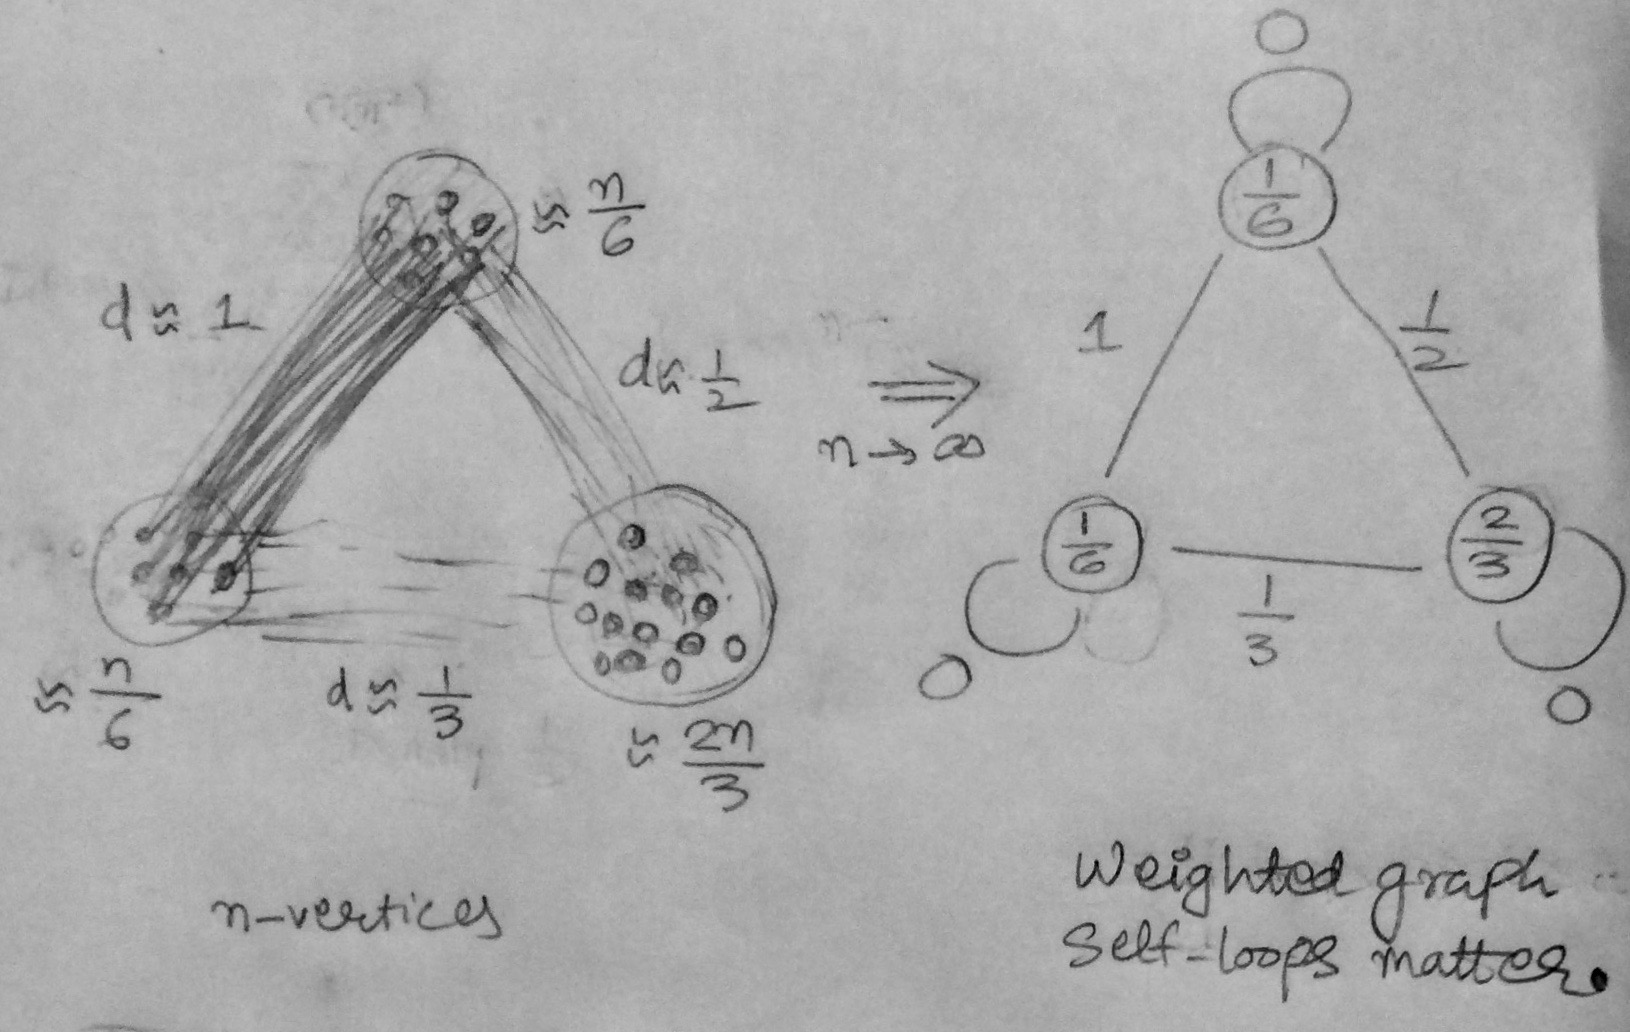
\includegraphics[totalheight=5cm]{./Images/Limit.jpg}
      \only<1>{\caption{$G_n$'s converge to a limit graphon}}
      \label{fig:limit}
    \end{figure}
    \only<1>{Precise definition using the cut-metric. Graphons can be much more complicated.}

    \begin{overlayarea}{\textwidth}{2cm}
      \begin{align*}
	  \only<2>{
	    \frac{\text{\# edges in } G_n}{\binom{n}{2}} \approx \frac{\left( \frac{n}{6} \right)^2 + \frac{n}{6}\frac{2n}{3}\frac{1}{2} + \frac{n}{6}\frac{2n}{3}\frac{1}{3}}{\frac{n^2}{2}}
      =  2(\frac{1}{6^2} + \frac{1}{2} \cdot  \frac{1}{6} \cdot \frac{2}{3} + \frac{1}{6} \cdot \frac{2}{3} \cdot \frac{1}{3})
	}
	  \only<3>{
	  \frac{\text{\# triangles in } G_n}{\binom{n}{3}} &\approx \frac{(\frac{n}{6})(\frac{n}{6})(\frac{1}{2}\cdot \frac{2n}{3} \cdot \frac{1}{3})}{n^3/6}
	  = 6 \cdot \frac{1}{6} \cdot \frac{1}{6} \cdot (\frac{1}{2} \cdot \frac{2}{3} \cdot \frac{1}{3})
	}
      \end{align*}
    \end{overlayarea}
  \end{frame}
  \begin{frame}
    \frametitle{subgraph counts}
    In fact if
    \begin{equation*}
      t'(F, G_n) \coloneqq \frac{\text{\# of occurances of }  F \text{ in } G_n}{\binom{n}{|F|}} 
    \end{equation*}
    then $lim_{n \to \infty} t'(F, G_n)$ exists for every finite graph $F$.
    
    \begin{block}{Why are these quantities important?}
    \pause
    \begin{equation*}
      t'(F, G) = \mathbb{P}(F = G'[k]) \approx \mathbb{P}(F = G[k])
    \end{equation*}
    \end{block}

    So if $G_n \to W$ then 
    \pause
    \begin{equation*}
      G_n[k] \xrightarrow{d} W[k] \quad \forall k \in \N
    \end{equation*}
    for some sequence of probability measures $\left( W[k] \mid k \in \N \right)$. 

    \pause
    In other words, \alert{$G_n[\infty] \xrightarrow{d} W[\infty]$} for some infinite random graph $W[\infty]$.
    
  \end{frame}

  \section{Conclusion}
  \begin{frame}
    \frametitle{Theorem}
    \begin{thm}[\cite{paper}]
      Let $G_n$ be a (non-random) sequence of graphs such that $|G_n| \to \infty$, the following are equivalent
      \begin{enumerate}
	\item $G_n$'s converge to $W$ in the cut-metric.
	\item There is an infinite random graph $W[\infty]$ so that $G_n[\infty] \xrightarrow{d} W[\infty]$.
      \end{enumerate}
      Moreover the map $W \to W[\infty]$ is a homeomorphism from the space of Graphons to the extreme points of the set of distributions of exchangeable random infinite graph.
    \end{thm}

    \printbibliography
\end{frame}
\begin{frame}
  Thank you.
\end{frame}

% etc
\end{document}

